% Table 1: example for a pair of species
% Table 2: model comparison across all species

\documentclass[12pt]{article}
\usepackage[utf8]{inputenc}
\usepackage{amsmath}
\usepackage{color,lineno,setspace,multirow}
\usepackage[sc]{mathpazo}
\usepackage{graphicx}
\usepackage[top=2.4cm,left=2.4cm,top=2.4cm,bottom=2.4cm,includefoot]{geometry}
\usepackage{rotating}

\begin{document}

\linenumbers 
\modulolinenumbers[1]

\textbf{Title:} Bringing Elton and Grinnell together: a quantitative framework to represent the biogeography of ecological interactions

\textbf{Authors:} Dominique Gravel$^{1,2,*}$, Ben Baiser$^{3}$, Jennifer A. Dunne$^{4}$, N\'eo
Martinez$^{5}$, Tommy Nyman$^{6}$, Timoth\'ee Poisot$^{2,7}$, Tomas Roslin$^{6}$, Spencer Wood$^{8}$, Daniel B. Stouffer$^{9}$, Jason Tylianakis$^{9}$\\

1: Canada Research Chair in Integrative Ecology. D\'epartement de
biologie, Universit\'e de Sherbrooke,  2500 Boulevard l'Universit\'e, 
Sherbrooke (Québec).  J1K 2R1\\

2: Qu\'ebec Centre for Biodiversity Sciences\\

3: University of Canterbury at Christchurch, School of Biological Sciences,\\

4: \\

5: \\

6:\\

7:\\

8:\\

9:\\

\textbf{Keywords:} networks, spatial ecology, co-occurrence, probability of interaction\\

\textbf{Words in the abstract:} 

\textbf{Words in the main text:} 

\textbf{Words in the legends:}  

\textbf{Figures:} 

\textbf{Tables:}     

\textbf{References:} 

\newpage
\doublespacing

%=============================================================================%
\section*{Abstract} 

\newpage


%=============================================================================%
\section*{Introduction}

Community ecology is defined in most textbooks as \emph{the study of the
interactions that determine the distribution and abundance of organisms}
(Krebs2001). Despite a general concensus on this definition (Scheiner2007), it
is surprising that most research on the variation of community structure has
focused mostly on the turnover of species composition (Anderson2011),
neglecting variation in the way they interact with each other (McGill2006).
Not surprisingly given this fact, biogeographers are still struggling to
figure out if interactions do impact species distribution (Wisz2012;
Kissling2012). There has been a step ahead with recent methodological
improvements accounting for interactions in species distribution models
(Pollock2014; Pelissier2013), but those remain nonetheless a 'species- based'
approach to communities where interactions are fixed covariates affecting
distribution. Here we plea for a more integrated approach of species and
interaction distribution.

The problem of community assembly is often formulated as \emph{how do we
sample a regional pool of species to constitute a local community?} This
question could be rewritten to adress the problem of network assembly, as
\emph{how do we sample a regional pool of interactions to constitute a local
interaction network?}. An illustration of this problem for a food web is
provided at Figure 1. The metaweb represents potential interactions among all
species that could be found in a given area. In this particular case, there
are 274 nodes, and 1077 links among plants, herbivores and parasitoids from
Northern Europe. An instance of a local community is also illustrated, with 44
nodes and 160 interactions. Only $51.2\%$ of all potential interactions are
realized. Our objective here is to provide a conceptual framework to explain
the sampling of the regional pool of interactions, along with a quantitative
method to predict it. The problem could be formalized by sequentially
understanding why only a fraction of the species are locally co-occurring, and
after why these species are interacting or not.

There are multiple causes to spatial turnover in community composition. The
first and most studied driver is the effect of variation in the abiotic
environment on species performance. Combined with specific responses in
demography, it generates variation among localities by locally selecting the
fittest species (Leibold2004). Stochasticity additionnaly plays a role, either
because of the inherently unpredictable nature of colonization and extinction
events, or because of strong non-linear feedbacks generating alternative
transients and equilibrium (Chase2007; Vellend2014). The analysis of community
turnover is usually performed with data represented in a table with rows
corresponding to sites (or measurements) and the columns to species. Beta-
diversity metrics quantify the variance of this community data (Legendre2005).
Traditionnal approaches rely on measures of the dissimilarity between
communities, using indices such as the Jaccard or the Bray Curtis measures of
dissimilarity. Recent methods decompose the total variation of the community
data into species and site contributions to beta diversity (Legendre2013).
Even though these methods compare whole list of species between sites, or
measurements, they remain fundamentally 'species-based' since they are all
based on the within column variation. None of them consider the variation of
associations (pairs or higher order motifs) explicitly.

The niche is by far the dominant concept to explain species distribution and
community assembly, from the local to the global scale. Following Hutchinson,
the niche is viewed as the set of environmental conditions allowing a
population to establish and maintain a population (see also Holt2009).
Community turnover arises following successive species replacement along an
environmental gradient, in agreement with a Gleasonian view of communities
(Gleason). The concept is straighforward to operationalize with species
distribution models, as it maps naturally on the available data (both
distribution and environmental data) and a vast array of statistical tools
representing it (e.g. Biomod, MaxEnt). It is however much harder to account
for ecological interactions in this approach (Peterson2011). These are often
viewed as externalities, constraining or expanding the range of environmental
conditions required for a species to maintain a population (Pulliam2000;
Soberon2007).

The network approach proposes a convenient formalism to represent the
structure of local communities. Species are represented as nodes and
interactions by links. The data could also be represented by matrices, with
each species in rows and columns, and the entries representing the occurrence
or the intensity of an interaction. Studies of network diversity are mostly
concerned by the distribution of the interactions within a location and not so
much by the variation among locations (Dunne2005; Bascompte2007; Ings2007;
Kefi2012). Network complexity is computed as the number of interactions in the
case of binary networks or interaction diversity in the case of quantitative
networks (Bersier2002). However, there is now evidence that ecological
interactions do also vary in space and time (Poisot2012; Trojelsgaard2015).
The variability of community structure in this situation arises from the
turnover of species composition, along with the turnover of the interactions
among pairs of species. The occurrence and intensity of interactions could
vary because of the environment, species abundance and higher order
interactions (Poisot2015a). The variation in community composition is often
independent of the variation of ecological interactions, suggesting these two
components of network variability respond to different drivers (Poisot2012).

Interestingly, the ecological network literature also has its own 'niche model' to
position a species in a community (Williams2000). The niche of a species in
this context represents the multidimentional space that could represent all of
its interactions. Each species is characterized by a niche position, an
optimum and a range over 3 to 5 different niche axes (Williams2000;
Eklof2013). The niche model has been successful at explaining the complexity
of a variety of networks, from food webs to plant-pollinator systems. The
conceptual framework is however limited to local communities and does not
provide any explanation to the turnover of network structure along
environmental gradients.

Here we adopt the view that a community structure is best represented as an
ecological network of interactions and develop a theory to explain its
turnover in space and time. We propose a new description of the niche that
integrates the effect of the environment on species distribution and on
ecological interactions. We first present the conceptual framework and then
formalize it mathematically with a probabilistic approach to the sampling of
the regional pool of interactions. We apply the framework to study the spatial
variation of host-parasite interactions across Europe. We find that the
variation of the environment causes both species and interaction turnover. The
network structures changes systematically across the latitudinal gradient,
with a peak of connectance at intermediate latitudes. At the pairwise level,
the statistical approach could be conceived as an interaction distribution
model. At the community level, the approach provides a likelihood based
method to compare different hypotheses of network turnover. 

%=============================================================================%
\section*{The integrated niche}

Correctly describing the niche is key to understand turnover in community
structure. Despite several attempts to refresh the conceptual basis of what
ecological niches are, ecologists have not moved far past the "n-dimensional
hypervolume" formalism introduced by Hutchinson. Despite its
intuitive interpretation and translation into species distribution models
(Boulangeat2012; Blonder2014), the concept has been constantly criticized
(Hardin1960; Peters1991; Chase2003; Silvertown2004; Soberon2007) and several
attempts have been made to expand and reinforce it.

Part of the problem surrounding the definition of the niche has been clarified
with the distinction between Eltonian and Grinnellian definitions (Chase2003).
The Grinnellian dimension of the niche is the set of environmental conditions
required for a species to maintain a population in a location. The Grinnellian
niche is the most intuitive to apply and is the conceptual backbone of species
distribution models. The Eltonian niche on the other hand is the effect of a
species on its environment. This aspect of the niche is well known by
community ecologists, but is trickier to turn into predictive models.
Nonetheless, the development of the niche model of food web structure
(Williams2000) and its parameterization (Williams2010; Gravel2013) made it
more operational.

These perspectives are rather orthogonal to each other and thus lead to
considerable confusion in the literature (McIntyre). Chase2003 attempted to
reconcile them in their definition of the niche: \textit{[The niche is] the
joint description of the environmental conditions that allow a species to
satisfy its minimum requirements so that the birth rate of a local population
is equal or greater than its death rate along with the set of per capita
effects of that species on these environmental conditions.} Their
representation merges zero-net growth isoclines figuring the Grinnelian niche
(when do the population persists) with impact vectors figuring the Eltonian
niche (what is the per capita impact). While this representation has been very
influential in community ecology at the local scale (the resource-ratio theory
of coexistence - Tilman1982), it remains impracticable at the large spatial
scale because of the difficulties to measure it. The absence of any
mathematical representation of the niche that could easily be fit to
ecological data perhaps explain why biogeographers are still struggling to
develop species distribution models taking into account ecological
interactions.

We propose to integrate the two perspectives of the niche with a visual
representation of both components. The underlying rationale is that, in
addition to the environmental constraints on demographic performance, any
organism requires resources to sustain its metabolic demand and reproduction.
Abiotic environmental axes are any non-consumable factors affecting the
demographic performance of an organism. Alternatively, the resource axes are
traits of the resources allowing interactions with the consumer. The niche
should therefore be viewed as the set of abiotic environmental factors (the
Grinnelian component) along with the set of traits (the Eltonian component)
allowing a sustainable population to establish and maintain at a location.
Accordingly, each species could be characterized by an optimal position in
both the environmental (x-axis) and the trait (y-axis) plane. The integrated
niche is then the hypervolume where interactions could occur and sustain a
population. This approach radically change the representation of the niche,
putting species distribution and ecological interactions in the same
formalism.

The limits of the niches could be independent of each other (as in the example
at Fig. 2), alternatively interact. For instance, the optimimal prey body size
for predatory fishes could reduce with increasing temperature (Lelong2015),
which would make diet boundaries functions of the environment. The other way
around, we could also consider that the growth rate of the predator could
change with the body size of the preys it feeds on, thereby altering the
environmental boundaries.

\newpage
%========================================================%
\section*{A probabilistic representation of ecological interactions networks in space}

We now formalize the integrated niche with a probabilistic approach to
interactions and distribution. We seek to represent the probability an
interaction between species $i$ and $j$ occurs at location $y$. We
define $L_{ijy}$ as a stochastic variable and are looking
at the probabilty this event occurs, $P(L_{ijy})$. The occurrence of an
interaction is dependent on the co-occurrence of species $i$ and $j$. This
argument might seem trivial at first, but the explicit consideration of this
condition in the probabilistic representation of ecological interactions will
prove fundamental to understand their variation. We thus define $X_{iy}$ as a
stochastic variable representing the occurrence of a species $i$ at location
$y$, and similarly $X_{ijy}$ the co-occurrence of species $i$ and $j$. The
quantity we seek to understand is the probability of a joint event:

%-----------------
\begin{equation}
\text{P}(X_{i,y},X_{j,y},L_{ij,y},)
\end{equation}
%-----------------

Or simply said, the probability of observing both species $i$ and $j$, and
an interaction from $i$ to $j$. This probability could be decomposed
in two parts using the product rule of probabilities:

%-----------------
\begin{equation}
P(X_{iy},X_{jy},L_{ijy})=P(X_{iy},X_{jy}|E_y)P(L_{ijy}|\mathbf{T},X_{iy},X_{jy},E_y)
\end{equation}
%-----------------

The left term is the probability of observing the two species co- occurring at
location $y$. It corresponds to the Grinnelian dimension of the niche. The
right term is a conditional probability, representing the probability that an
interaction occurs between species $i$ and $j$, given their set of traits
$\mathbf{T}$ and they are co- occurring. It is referred as the metaweb and
corresponds to the Eltonian dimension of the niche described above. We will
see below how this formalism could be directly fitted to empirical data. But
before turning to an application, we will discuss the interpretation of
different variants of these two terms.

\subsection*{Variants of co-occurrence}

There are several variants to the co-occurrence probability representing
different hypotheses about the temporal and spatial variation in network
structure (see the explicit formulations at Table 1). The simplest model
relates co- occurrence probability directly to the environment, $P(X_{ijy} |
E_y)$. In this situation there is no underlying assumption about the
ecological processes responsible for co-occurrence. It could arise because of
the impact of ecological interactions on distribution (Pollock2014) or
alternatively because of share environmental requirements. In the former case,
species are not independent to each other and the conditional occurrence must
be accounted for explicitlty, $P(X_{ijy} | E_y) = P(X_i | E_y, X_j)P(X_j |
E_y)$. In the later case, species are independent and only the marginal
occurrence must be accounted for, $P(X_{ijy} | E_y) = P(X_i | E_y)P(X_j |
E_y)$.

The co-occurrence probability itself could be dependent on ecological
interactions. Direct pairwise interactions such as competition, facilitation
and predation have long been studied for their impact on co-distribution (such
as in the cases studied by Diamond1976, Connor1980, Gotelli2000 etc..). Second
and higher order interactions (e.g. trophic cascade) could also impact co-
occurrence. Co-occurrence in ecological networks is however a topic of its
own, influenced by the degree distribution and species richness
(Cazelles2015). Almost only first order and second order interactions do
impact co-occurrence. The covariance of interacting species to an
environmental gradient also influences co-occurrence (Cazelles2016). Because
of the complexity of relating co-occurrence to the interaction network
structure, we  will focus here on the variation of interactions and not on the
distribution, and leave this issue for Discussion and future research.

\subsection*{Variants of the metaweb}

There are also variants of the metaweb. First, most documented metawebs have
thus far considered that ecological interactions are deterministic, not
probabilistic (e.g. Havens1992; Woods2015). Species are assumed to interact if
they are found together in a location, independently of their abundance and
the environment. In other words, $P(L_{ijy}) = 1$ if $X_{ijy} = 1$, and 0
otherwise. This approach might be a reasonnable approximation when the
sampling and inference scales are large enough so that probabilities of
observing at least one interaction converges to unity and that the only
variation of networks considered arises from species distribution.

Ecological interactions could also vary with the environment, such as
$P(L_{ijy} | E_y)$. Although it is not common to see a conditional
representation of ecological interactions, experimental studies of pairwise
interactions revealing their sensitivity to the environment are common (REF).
For instance, it has been documented that the predation risks of shorebirds do
vary at the continental scale, from the south to the north (REF). The effect
of the environment on interactions propagate up the community and influence
network structure (REF).

\newpage
%========================================================%

\section*{Application: continental-scale variation of host-parasite community structure}

In this section we provide an illustration of the framework with an empirical
dataset of host-parasitoid networks sampled throughout continental Europe
along a south-north gradient. The analysis targets networks composed of
willows (genus Salix), their galling insects, and the natural enemies of these
gallers. The questions we address with the framework and the dataset are: i)
how much variation in the network structure is there across the gradient and
ii) what is the primary driver of network turnover across the gradient?

\subsection*{Data}  

Communities of both willows and gallers are species-rich and widely
distributed, with pronounced variation in community composition across space.
The genus Salix includes over 400 species, most of which are shrubs or small
trees (ref). The genus is common in most habitats across the Northern
Hemisphere (ref). Willows support a highly diverse community of herbivorous
insects, and one of the main herbivore groups in this system are gall-inducing
sawflies (Hymenoptera: Tenthredinidae: Nematinae: Euurina (ref). Gall
formation is induced by sawfly females during oviposition, and gall formation
includes marked manipulation of plant chemistry by the galler (ref). The enemy
community of the gallers includes nearly 100 species belonging to 17 insect
families of four orders. These enemies encompass both inquilines and
parasitoids: inquiline larvae (Coleoptera, Lepidoptera, Diptera, and
Hymenoptera) feed primarily on gall tissue, but typically kill the galler
larva in the process. Parasitoid larvae (representing many families in
Hymenoptera) kill the galler larvae by direct feeding (REF). In terms of
associations between the trophic levels, phylogeny-based comparative studies
have demonstrated that galls represent "extended phenotypes" of the gallers,
meaning that gall form, location, and chemistry is determined mainly by the
galling insects and not by their host plants [ref]. Because galler parasitoids
have to penetrate a protective wall of modified plant tissue in order to gain
access to their victims, gall morphology has been inferred to strongly affect
the associations between parasitoids and hosts (ref, ref). Thus, the set of
parasitoids attacking each host is presumptively constrained by the form,
size, and thickness of its gall.

Local realizations of the willow–galler–enemy network were reconstructed from
samples collected between 1982 and 2010. Plant galls were collected by J.P.
Kopelke during this period at 374 sites across Central and Northern Europe.
Sampling was conducted in the summer months of June and/or July, during the
latter stages of larval development. Galler species were identified on the
basis of willow host species and gall morphology, as these are distinct for
each sawfly species. At each site, galls were randomly collected from several
willow individuals in an area of about 0.1-0.3 km2. Most sites were visited
only once, with a total of 641 site visits across the 374 sites. GPS
coordinates were recorded for each location and the annual mean temperature
and annual precipitation were obtained from WorldClim. While other covariates
could have been considered, we figured that they are representative of the
most important axes of the European climate, and more easily
interpretable than reduced variables obtained by a PCA,

The methods used for rearing natural enemies from the galls have been
previously described by e.g. [ref, ref]. In brief, galls were opened to score
the presence of galler or parasitoid/inquiline larvae. Enemy larvae were
classified to preliminary morphospecies, and the identity of each
morphospecies was determined by connecting them to adults emerging after
hibernation. The galls were reared by storing single galls in small glass
tubes (Kopelke 1985a, 1994a, 1999, 2003a, b). Hibernation of galls containing
parasitoids took place either within the glass tubes or between blotting paper
in flowerpots filled with clay granulate or a mixture of peat dust and sand.
These pots were stored over the winter in a roof garden and/or in a climatic
chamber. In most cases, the matching of larval morphospecies with adult
individuals emerging from the rearings allowed the identification of the
natural enemies to the species level. Nonetehless, in some cases, individuals
could only be identified to one of the (super)families Braconidae,
Ichneumonidae, and Chalcidoidea. This was particularly the case when only
remains of faeces, vacant cocoons of parasitoids, and/or dead host larvae were
found, as was the case when parasitoids had already emerged from the gall. As
a result, the largest taxon in the data set, “Chalcidoidea indeterminate,”
represents a superfamily of very small parasitoids that are hard to
distinguish.

In total, the sampling targeted 52 Salix taxa, yielding 146,622 galls for
dissection and rearing. These galls represented 96 galler species, and yielded
42,133 individually-identified parasitoids and inquilines. Of these, 25,170
(60\%) could be identified to the species level. Overall, 126 parasitoid and
inquiline taxa were distinguished in the material. Data on host associations
within subsets of this material have been previously reported by (Kopelke ref
ref b) and by Nyman et al. 2007, whereas the current study represents the
first analysis of the full data set from a spatial perspective.

\subsection*{Analysis}  

Computing the probability of observing an interaction involves fitting a set
of binomial models and collecting their estimated probabilities. We considered
second-order generalized linear models for the sake of the illustration, but
more sophisticated fitting algorithms (e.g. GAM or Random Forest) could be
used as well, as long as the algorithm can provide an estimated probability
for each observation. The data consists of a simple (albeit large) table with
the observation of each species, $X_i$ and $X_j$, their co-occurrence,
$X_{ij}$, the observation of an interaction $L_{ij}$, and environmental co-
variates. There is one row per pair of species per site. We considered that an
absence of a record of an interaction between co-occurring species at a site
means a true absence.

We compared three models for the co-occurrence probability. The first model
fits directly the co-occurrence probability conditional
on the local environment, $P(X_{ijz}|E_z)$. This model therefore does not make any
hypothesis about the mechanisms driving co-occurrence for any given
environment and use the information directly available in the data. The second
models consider independent co-occurrence of species. In this case, we fit
independently $P(X_{iz}|E_z)$ and $P(X_{jz}|E_z)$ and take their product to
derive co-occurrence probability. This model should be viewed as a null
hypothesis with respect to the first model since their comparison reveals if
there is significant spatial association of the two species once considering
the response to the environment (Cazelles2016). Finally the third model
considers that co-occurrence probability is independent of the environment and
thus constant throughout the landscape.  In other words, $P(X_{ijz})$ is
obtained by simply counting the number of observed co-occurrences, divided by
the total number of observations. The comparison between the first and third
model allows testing the hypothesis that co-occurrence is conditional on the
environment. Whenever the environment is included as a co-variate in the glm,
we considered a second-order polynomial response for both the temperature and
precipitations. There are consequently 5 parameters for the first model when
fitting a given pair of species, 10 parameters for the second model and only 1
for the third model.

Following the same logic, we compared three models for the interaction
probability. The first model fits the interaction probability conditional on
the local environmental variables, $P(L_{ijz}|E_z,X_i,X_j)$. Consequently, the
model was fitted on a subset of the data, when the two species are found co-
occurring. The second model fits the interaction probability independently of
the local environmental variables, $P(L_{ijz}|X_i,X_j)$. It corresponds to the
number of times the two species were observed interacting when co-occurring,
divided by the number of times they co-occurred. The third model is an extreme
case performed only to test the hypothesis that if two species are found to
interact at least once, then they should interect whenever they co-occur,
$P(L_{ijz}|X_i,X_j)=1$. While not necessarily realistic, this model tests an
hypothesis that is commonly done in the representation of local networks from
knowledge of a deterministic metaweb (such as in Havens1992; Piechnik2008;
Wood2015). There are consequently 5 parameters for the first model, a single
parameter for the second model and no parameter to evaluate for the third
model (the interaction probability is fixed by hypothesis).

The different models were fitted to each pair of species and the fitted
probabilities were recorded. The joint probability $P(L_{ij},X_i,X_j)$ was
then computed from Eq. 2 and the likelihood of each observation was computed
as $L(\theta|D) = P(L_{ij},X_i,X_j)$ if an interaction was observed and
$L(\theta|D) = 1 - P(L_{ij},X_i,X_j)$ if no interaction was observed. The log-
likelihood was summed over the entire dataset to compare the different models
by AIC. Not surprisingly, it was impossible to compute this model for a very
large number of pairs of species because they never co-occurred. These pairs
were removed from the analysis because the co-occurrence probability is null
and we have no information for the interaction probability. The reported
likelihood across the entire dataset is summed over all pairs of species that
were observed co-occurring at least one time. We considered separately the
salix-galler and the galler-parasitoid interactions. 

Finally, we used the full model (both the co-occurrence and the interaction
are conditional on the environment) interpolate species
distribution and the interaction probability across the entire Europe. We 
reconstructed the expected network for each location in a 1km X 1km grid. We
then after computed the probabilistic connectance following Poisot2015b.

All of the data are openly available in the database \emph{mangal}
(Poisot2015) and all R scripts for querying and pre-processing the data, along
with the analysis are provided in supplementary material.

\subsection*{Results}  

We start with an example for a single pair of species that we selected because
of a sufficiently large number of times they were found co-occurring ($N_{ij}
= 41 $). Despite the extent of the sampling, many pairs of species are found
co-occurring only a few times, making it hard to evaluate interaction
probabilities with a reasonnable confidence interval. This particular example
involves the interaction between \textit{Phyllocolpa plicalapponum} and
\textit{Pediobius saulius}, two fairly abundant species, observed respectively
$N_i = 53$ and $N_j = 129$ times across the 374 sites. These two species are
found interacting with marginal probability $P(L_{ij}) = 0.73$, which means
they were found interacting at 30 different locations. The model comparaison
(Table 1) reveals that the interaction probability conditional on the co-
occurrence better explain the distribution (Model 1 vs Model 2). The
probabilistic representation of the metaweb yields a much better fit to the
data than the deterministic version. When the two species co-occur, the
occurrence of the interaction is insensitive to the environment (Model 2 vs
Model 3). Alternatively, climatic variables significantly impact co-
occurrence (Model 3 vs Model 4). The neutral model performs worst than the
non-random co-occurrence model (Model 3 vs Model 6). The full model reveals
that the greatest interaction probability occurs at intermediate temperature
and precipitations, simply because this is where the two species are found co-
occurring the most often (Fig. 3). The co-occurrence and the interaction
probabilities could be represented in space, where we find that the highest
interaction probability occurs in central Europe (Fig. 4).

We did evaluated each model for all pairs of species in order to better
understand the large scale drivers of network turnover. Salix-gallers and
gallers-parasitoids were analyzed separately (Table 2). The results are
comparable, albeit some very minor details. We do find that across all pairs
of species, the probabilistic representation of interactions again does better
than the deterministic (Model 1 vs Model 2). Interactions do not happen
systematically whenever the two species are found co-occurring, meaning that
the stochastic nature of interactions contribute to network variability in
addition to species turnover. There are 1077 recorded pairs of interactions,
with only 224 of them occurring less than 5 times. Out of these 224
interactions, only 77 are found systematically whenever the two species do
co-occur. Even though interactions are better represented probabilistically,
the two environmental variables that were considered are pretty poor
predictors of their occurrence (Model 2 vs Model 3). Not surprisingly, the
likelihood increases for both types of interactions when the environment is
considered. The extra number of parameters however exceed the gain in
likelihood, and therefore the best model excludes the effect of the
environment.

According to the log-likelihood only, the co-occurrence is non-neutral for salix-
galler interactions, while it is neutral for the galler-parasitoid
interaction. However, the gain in log-likelihood for the neutral model of galler-
parasitoid co-occurrence is inferior to the extra number of parameters (twice
as many since two species distribution models are fitted instead of just one),
which has for consequence that the best model according to AIC has non-random
co-occurrence (Model 3 vs Model 6), for both types of interactions.

The approach we present not only has implications for understanding the
biogeography of pairwise interactions and interaction networks, but also the
quality of the evaluation of metawebs. We investigated the reliability of the
estimated metaweb across the entire dataset. As mentionned above, across the
32 412 pairs of species, only 1077 pairs are interacting at least at a single
location, for a connectance of 0.03. However, only 8437 species are found co-
occurring at least one time across all locations. There are consequently 23975
gaps of information in the metaweb (74.0\% - see Fig. 5). Given that we do not
know if the non co-occurring species do indeed co-occur, it means that a more
appropriate estimate of connectance would be $C = 1077/8437 = 0.128$. This
result reveails that the evaluation of the sampling quality of ecological networks is a
problem on its own that worths further attention.

Once we selected the best model (model 3, Table 2), we were able to
reconstruct the expected species richness across Europe, along with the most
likely network for each location, and therefore map the expected distribution
of network properties (Fig. 6). We simply considered connectance, as it could
be easily computed from probablistic networks (Poisot2015b) and is also a good
proxy for many other network properties (Poisot2014). The diversity of Salix
tends to increase toward boreal areas, and we consequently find a peak in
diversity in northern Europe. The distribution of the expected number of
interactions follows the distribution of species richness, but not at the same
rate. Consequently, connectance is peaking in central Europe and in
England.


\newpage
%========================================================%
\section*{Discussion}

\textbf{Summary of the framework}\\
% 	- concept of integrated niche
% 	- visual
% 	- explored it with network data
% 	- useful to characterize not only the turnover in community composition, but also its structure
% 	- useful to understand spatial variation of processes such as top-down control, as well as community build-up. 

\textbf{Toward interaction distribution models} \\
% 	- different approach, based on the variance, to investigate the network turnover
% 	- much closer in spirit to species distribution models


\textbf{What are the drivers of network variation in space?}\\
% 	- environment mostly affect co-occurrence
% 	- here links do not vary so much
% 	- we know that some interactions vary with the environment
% 	- perhaps we haven't had the appropriate covariates
% 	- new investigations with other systems will be required to challenge this result 

\textbf{Forecasting network structure under global change}\\

% Quantifying the uncertainty and the variability of network structure

\textbf{Investigating the realized niche and the impact of biotic interactions on distribution}\\
% 	- havent look much at the drivers of co-occurrence, single took them granted from the data
% 	- many species are not different from the neutral
% 	- raise the question, once accoutning for the environment, are there true effects of interactions on distribution
% 	- for sure the analysis raise intersting points
% Provided that interactions do matter, could derive SDM
% 	- invert the problem
% 	- needs an hypothesis for 
% 	- could be derived from simple models such as
% 	- or from explicit rules such as


\textbf{Guidance for empirical studies}\\
% Ecological networks are known to be extremely sparse, \emph{i.e.} having far
% more absences of interactions that they have interactions. These absences of
% interactions, however, can come from different sources. The fact that unequal
% sampling at the local scale can affect our understanding of network structure
% is well documented \parencite{Martinez1999}. However, in a spatial context,
% some interactions may be undocumented because the species involved have
% never been observed in co-occurence. Although these are reported as a lack
% of interactions, in actuality we cannot make inference about them seeing
% that they have never been observed: it is possible that this interaction
% may happen should the two species co-occur. A second category of absences
% of interactions are those that are reported after multiple observations of
% species co-occurence. However, so as to have a confidence in the fact that the
% probability of an interaction is low, extensive sampling (that is, several
% co-occurences) is needed. Generally, our confidence that the interaction
% is indeed impossible will increase when the number of observations of the
% species pair. Seeing that this is essentialy a Bernoulli process (what is
% the probability that the species will interact given their presence), the
% breadth of the confidence interval is expected to saturate after a fixed
% number of observations, which can be set as a treshold above which a species
% paier has been observed "often enough".


% Conclusion



\newpage




%========================================================%
\section*{Conclusion}

\textbf{Research agenda on probabilistic interactions}\\
\begin{itemize}
	\item Need a new type of data
	\item Need to investigate the reliability of interactions
	\item From interaction probabilities to a distribution of network properties 
	\item Deeper investigations of the environmental dependence of interactions
	\item Trait-based approach to interactions
	\item The effect of interaction on co-occurrence
\end{itemize}

\newpage






%========================================================%
\section*{Acknowledgements}
This is a contribution to the working groups \emph{Networks over ecological
gradients} (Santa Fe Institute) and \emph{Continental-scale variation of
ecological networks} (Canadian Institute for Ecology and Evolution). 
\newpage

%========================================================%

\newpage
%========================================================%
\section*{Figure legends}

%------------------------
\subsection*{Figure 1}
\textbf{Non-random sampling of the metaweb}. 
Network assembly could be viewed as a sampling process of the regional pool of
potential interactions. Species are sampled first (indicated by colored nodes)
and among the present species in the local network, only some interactions are
occurring (indicated by colored links). The challenge we address with the
quantitive framework proposed is to adequately characterize this sampling
process. The sampling of the metaweb is illustrated with a local interaction
network among Salix, gallers and parasitoids. Here, the metaweb was
constructed by aggregating observed interactions across 374 local networks.
The color nodes represent the species that were found in the most diverse of
these 374 local networks.

%------------------------
\subsection*{Figure 2}
\textbf{Visual representation of the integrated niche}. 
We represent visually the integration between two views of the niche. In
biogeography, the niche is considered the set of environmental conditions
where the intrinsic growth rate $r$ is positive. The horizontal axis
represents an environmental gradient impacting the growth of the focal species
(in red). The location of the different species along this gradient represent
their optimum, and the vertical dotted lines represent the limits of the
[Grinnelian] niche of the focal species. In food web ecology, the [Eltonian]
niche represents the location of a species in the food web, as determined by
its preys and its predators. The vertical axis represents a niche gradient,
presumably a trait such as body size. The location of each species along this
gradient represent their niche position. The focal species will feed on the
different preys whose niche location falls within a given interval around the
optimum, represented by the horizontal dotted lines. The integrated niche
[Grinnelian \& Eltonian] corresponds to the square in the middle where an
interaction is possible. According to our probabilistic framework, the central
square represents the area where the joint probability of observing
interactions and co-occurrence is positive.

%------------------------
\subsection*{Figure 3}
\textbf{Probabilistic representation of the interaction probability between a leaf galler (\textit{Phyllocolpa plicalapponum}) and a parasitoid (\textit{Pediobius saulius}) across a temperature and a precipitation gradient}. The representation is based on predictions from model 3 (see Table 1). For the left panel: open circles represent the absence of both species or of an interaction, the closed circles represent co-occurrence and other symbols the occurrence of only one of the two species. For the other two panels the open circles represent co-occurrence but an absence of interaction and the closed circles represent the occurrence of an interaction. 

%------------------------
\subsection*{Figure 4}
\textbf{Probabilistic representation of the interaction probability between a leaf galler (\textit{Phyllocolpa plicalapponum}) and a parasitoid (\textit{Pediobius saulius}) across Europe}. 

%------------------------
\subsection*{Figure 5}
\textbf{Representation of the A) metaweb and B) gaps of data in the metaweb}. The salix and gallers were regrouped as 'victims' for the sake of the illustration, as the gallers and the parasitoids were regrouped as 'ennemies'. 

%------------------------
\subsection*{Figure 6}
\textbf{Mapping the distribution of species richness, the number of links and connectance across Europe}. The representation is based on predictions from model 3 (see Table 2).  

\newpage


%========================================================%
%------------------------
\subsection*{Figure 1}

\begin{figure}[ht!]
\centering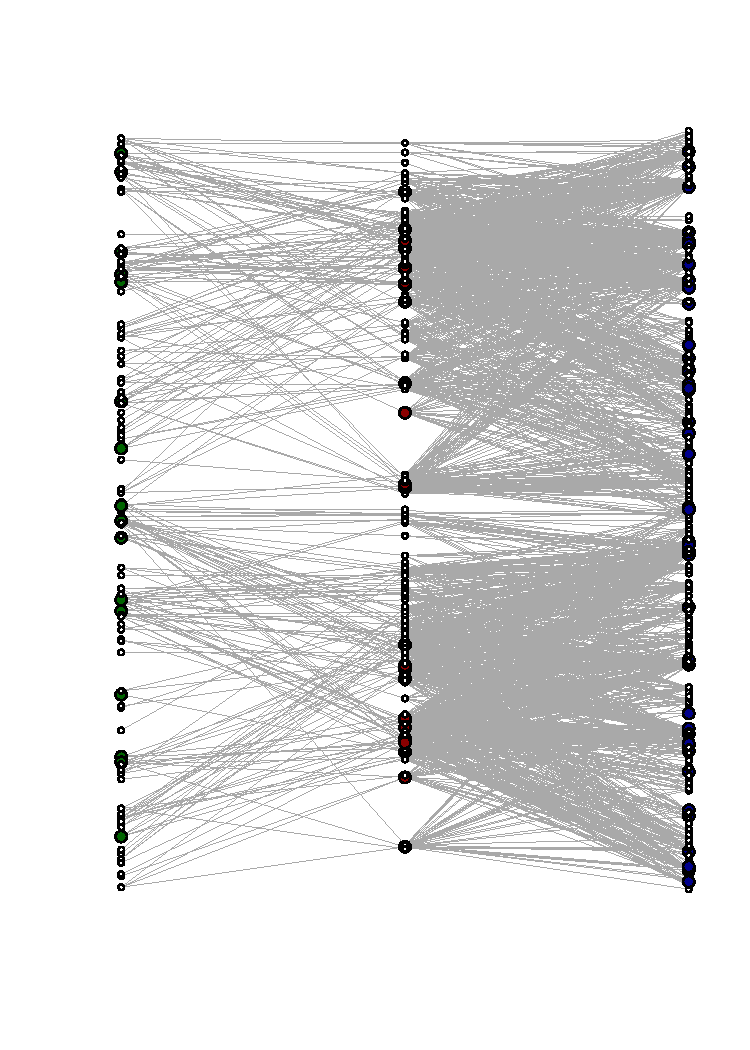
\includegraphics[width=0.8\textwidth]{figures/mw_sampling}
\end{figure}

\newpage

%------------------------
\subsection*{Figure 2}

\begin{figure}[ht!]
\centering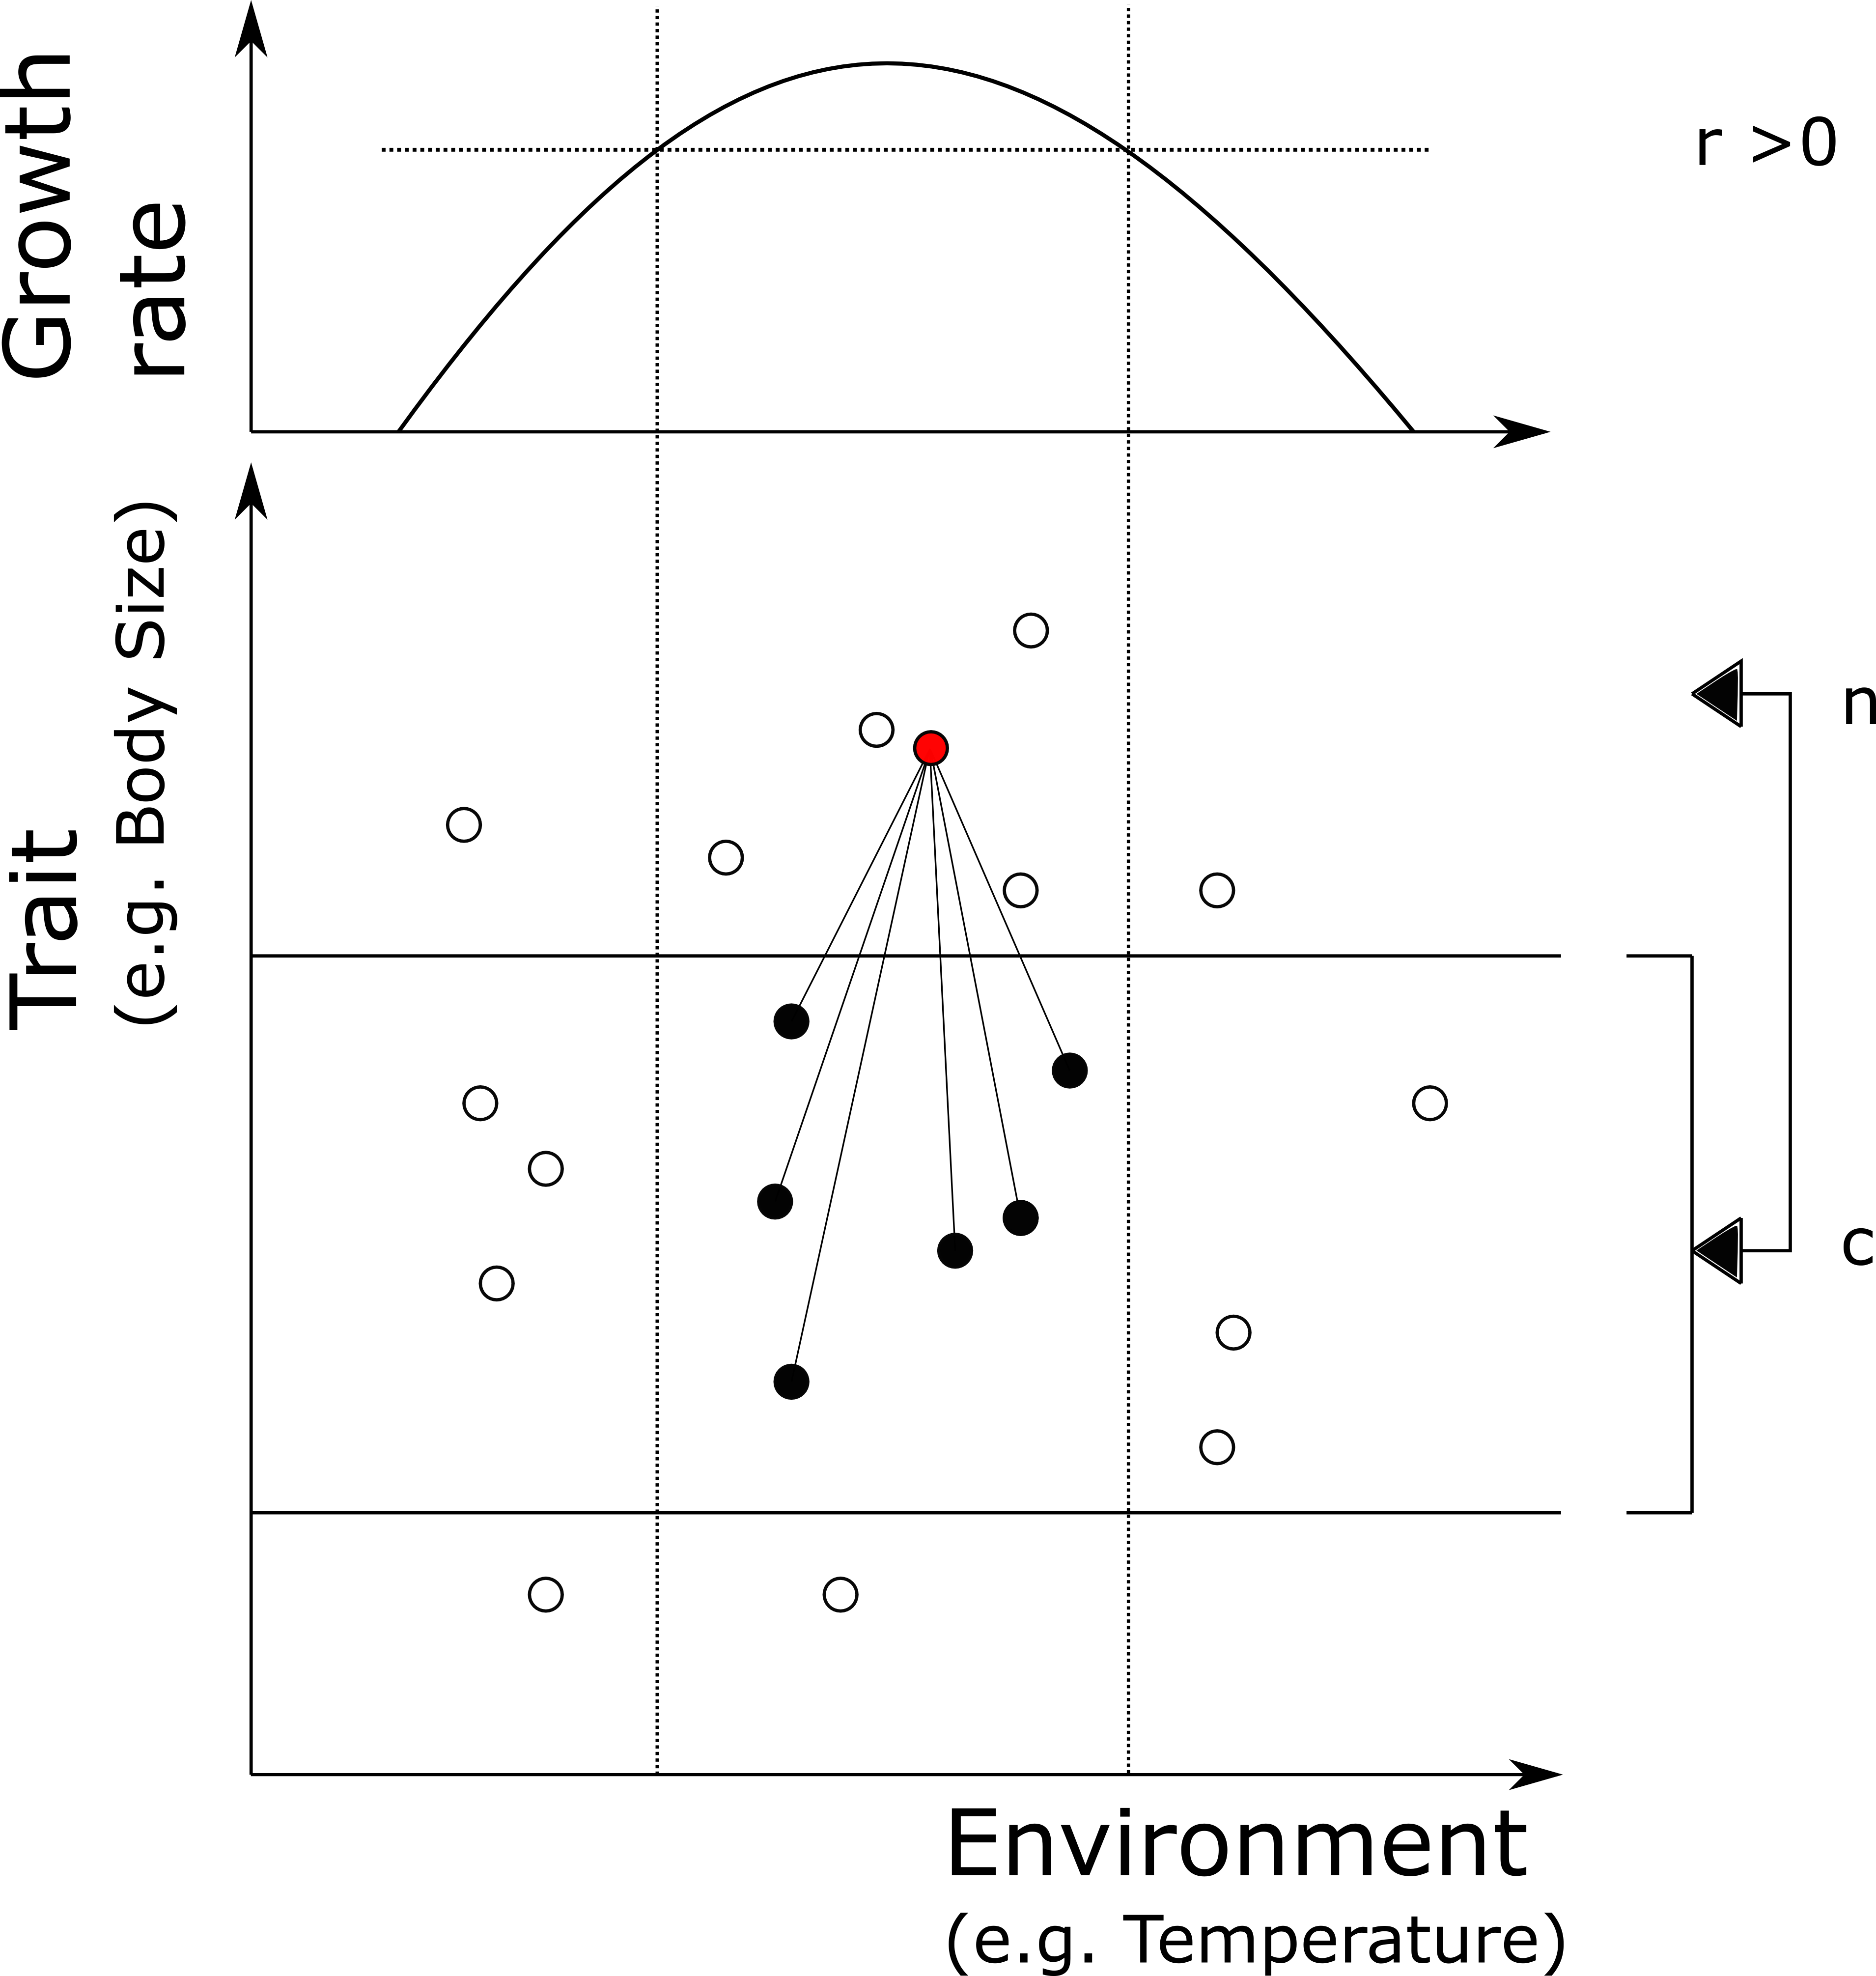
\includegraphics[width=0.8\textwidth]{figures/integrated_niche}
\end{figure}

\newpage

%------------------------
\subsection*{Figure 3}

\begin{figure}[ht!]
\centering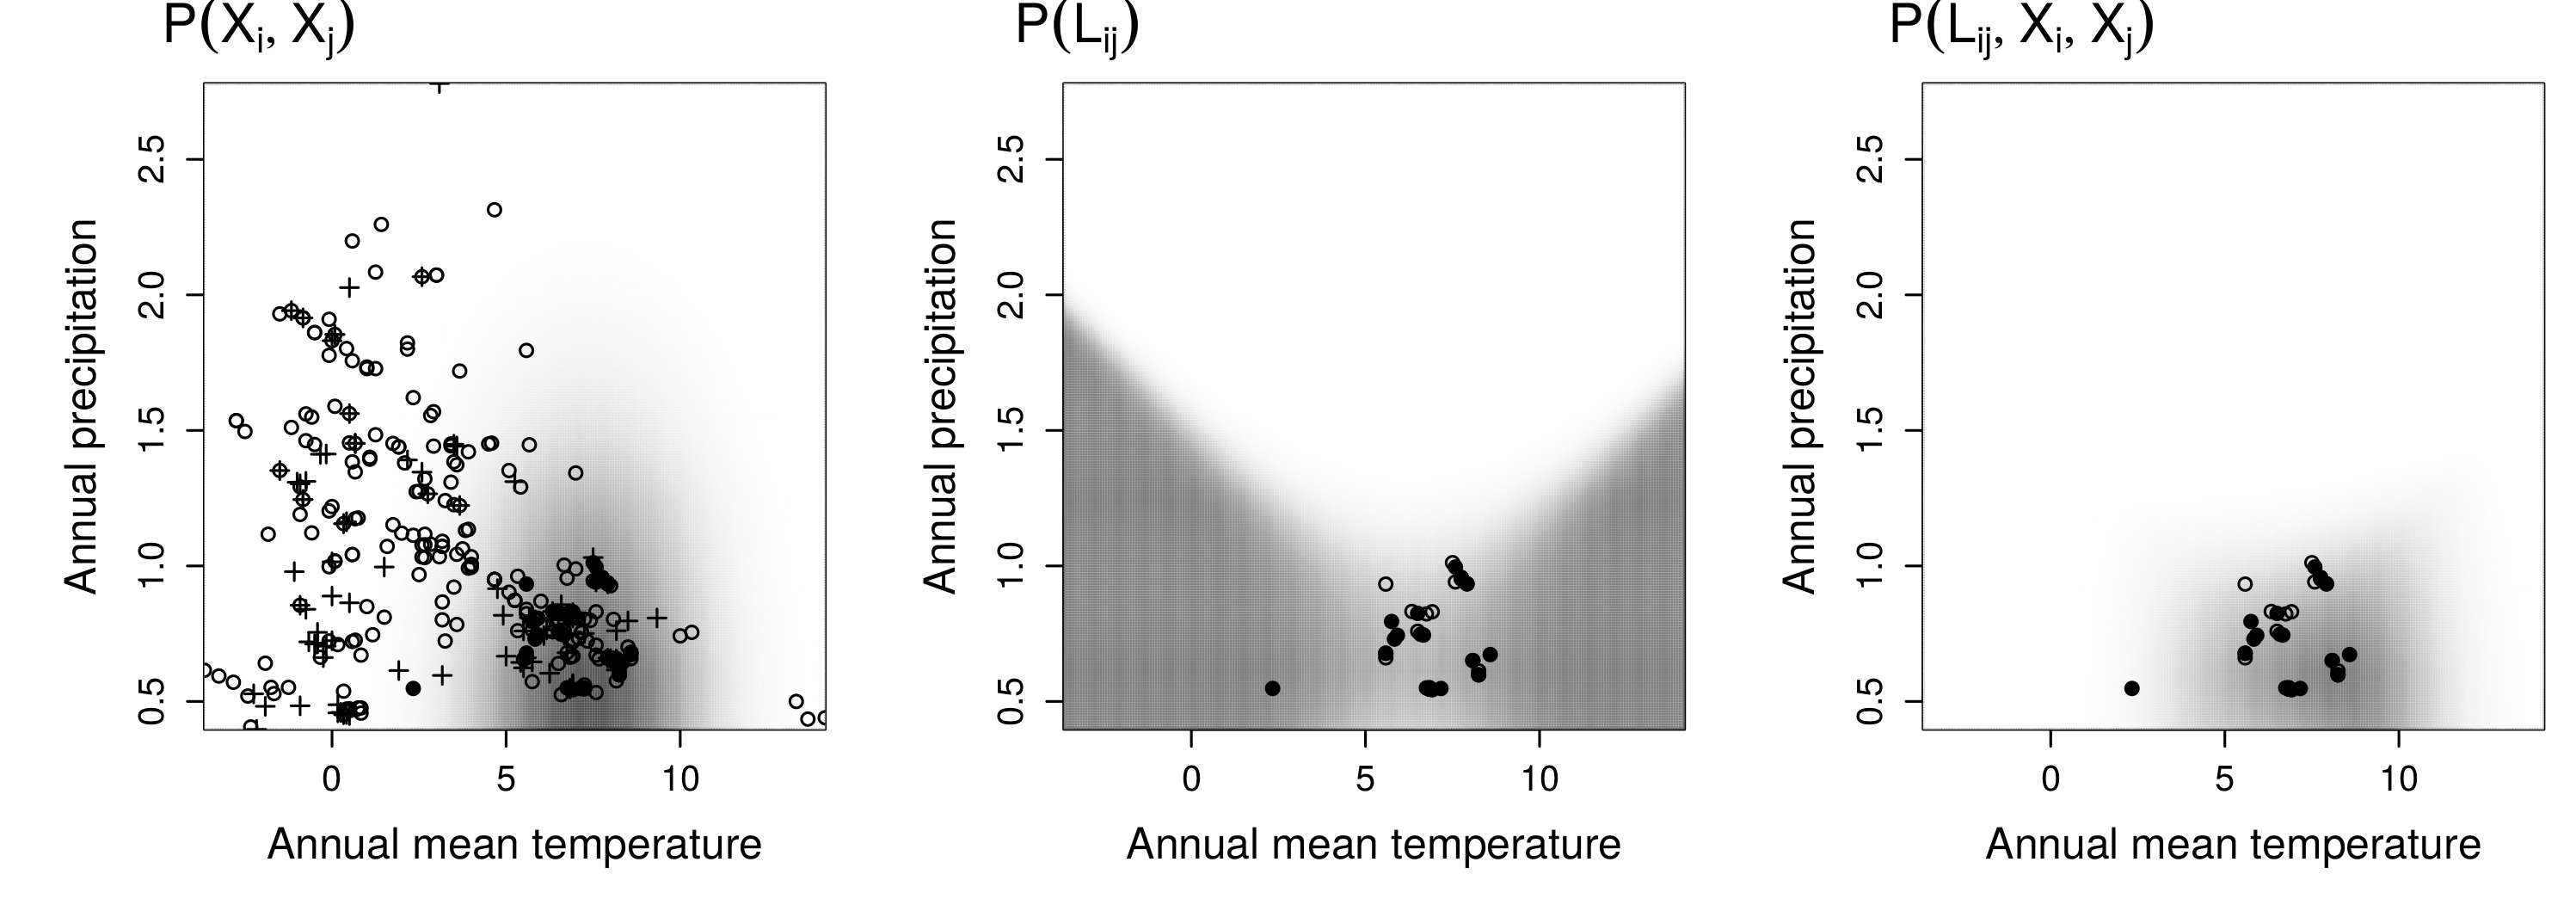
\includegraphics[width=0.8\textwidth]{figures/example_pair}
\end{figure}

\newpage

%------------------------
\subsection*{Figure 4}

\begin{figure}[ht!]
\centering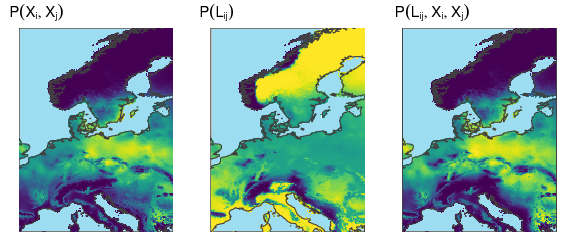
\includegraphics[width=0.8\textwidth]{figures/map_pair}
\end{figure}

\newpage

%------------------------
\subsection*{Figure 5}

\begin{figure}[ht!]
\centering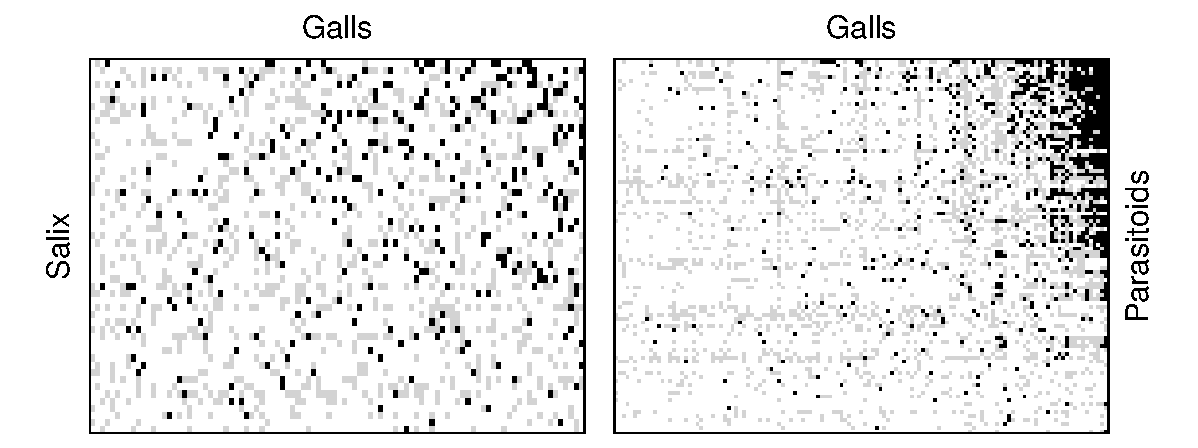
\includegraphics[width=0.8\textwidth]{figures/mw_holes}
\end{figure}

\newpage

%------------------------
\subsection*{Figure 6}

\begin{figure}[ht!]
\centering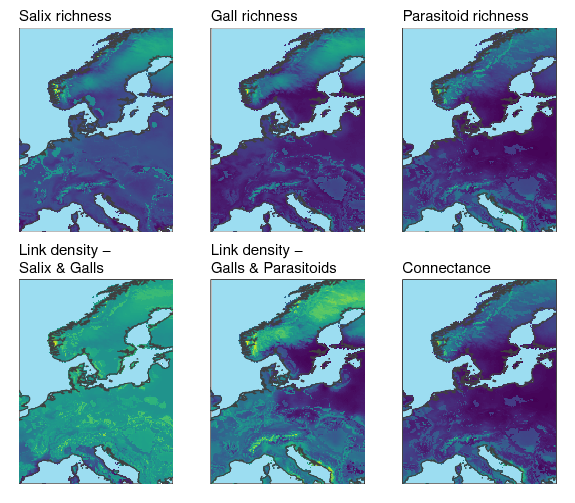
\includegraphics[width=0.8\textwidth]{figures/map_connectance}
\end{figure}

\newpage


%========================================================%
\end{document}